\documentclass[11pt,a4paper,oneside]{article}
\usepackage{ucs}
\usepackage{a4wide}
\usepackage[utf8x]{inputenc}
\usepackage{listings}
    \lstset{numbers=left, numberstyle=\tiny, numbersep=5pt,frame=leftline}
    \lstset{language=Java} 
    \lstset{basicstyle=\small,tabsize=4,extendedchars=false,columns=flexible}
%    \lstset{keywordstyle=\ttfamily\bfseries}
    \lstset{keywordstyle=\bfseries}
    \lstset{identifierstyle=\ttfamily}
    \lstset{stringstyle=\rmfamily,showstringspaces=false}
    \lstset{commentstyle=\rmfamily\itshape}
\usepackage{graphicx}
\usepackage{geometry}
\geometry{a4paper,left=20mm,right=20mm, top=1cm, bottom=2cm, includeheadfoot}
\usepackage[pdfborder={0 0 0}]{hyperref}

\title{BONAPARTE DSL Tutorial}
\author{Michael Bischoff}
\begin{document}
\maketitle
\begin{abstract}
This document provides a tutorial for the Bonaparte DSL grammar. While the grammar is independent of the generated code language,
the tutorial will often reference generated Java specific aspects, simply because currently Java is the only implemented target language
and splitting this information into a different document would complicate the understanding.
\end{abstract}

\section{Main Concepts}
The main concepts of the Bonaparte DSL are packages and classes. While the syntax of the DSL is close to Java, there are also a lot of differences.
For example, the source code directory of a file is not determined by it's contents. It is recommended however that you define some project specific
conventions.

The main focus of the DSL is to define (and generate) classes for data transfer objects (DTOs), which are transmitted across servers.
Therefore, an emphasis is on plausibility checks and description of transferred data. There are for example different data types for ASCII strings
and Unicode strings.

There is a ``native'' serialization format defined, which supports all the features defined, there are however also different formats supported,
such as Java serialization, XML, CSV and even fixed width interfaces (required for languages such as COBOL). Therefore, the Bonaparte DSL
is ideal to work in cross-language environments.


\section{A first example}
Before digging into too much detail, let's start with a small example.  You need an Eclipse IDE (release 4.2 Juno) and special plugins
(available at \url{https://www.jpaw.de/eclipse/juno/site.xml}) to follow the examples.

Create a new Java project, create a new source folder (for example {\ttfamily src/main/bon}), and create a new file with extension {\ttfamily .bon},
for example {\ttfamily tutorial1.bon}. If everything is set up correctly, Eclipse will ask ``Do you want to assign the XText Nature to the project
 {\it{ (your project name)}}?''.
It is important to say ``Yes'' here, only then the specific editor features will be available.

Create a package and a class in it. In Bonaparte, scopes are consistently defined by curly brackets. You can define multiple packages in a single source file.
As in Java, packages can contain components, separated by a dot.

\vspace{2mm}
\begin{center}
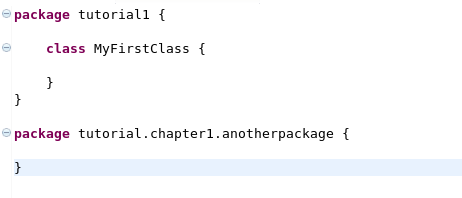
\includegraphics[scale=0.5]{images/tut1-001.png}
\end{center} 

You can observe the following:
\begin{itemize}
  \item Syntax highlighting. Keywords such as {\ttfamily package} or {\ttfamily class} are displayed in a different color,
  comparable to Java syntax highlighting.
  \item Source folding. You see small encircled minus signs at the left side. Click on them to collapse or expand the corresponding scope areas.
  \item Auto-completion.  If you type {\ttfamily packa} and then press ctrl-space, Eclipse will auto-complete the keyword {\ttfamily package}.
  In case of multiple possibilities, you will get a popup window with all expansions valid in the current context. 
  \item Online syntax checking. Enter a class name which starts with a lower case letter.  
\vspace{2mm}
\begin{center}
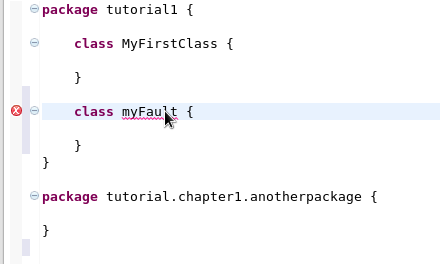
\includegraphics[scale=0.5]{images/tut1-002.png}
\end{center} 
    If you move the mouse above the keyword underlined with the way red line, Eclipse will show a tooltip with the explanation
     ``Class names should start with upper case letters''. 
 
\end{itemize}

Delete the class with the incorrect name. We want to add some fields to the class {\ttfamily MyFirstClass} now. As a type keyword, Bonaparte supports all
primitives and their boxed equivalents of Java (which, for the Java code generator, map exactly to their corresponding Java equivalent), plus the following additional types:
 
\begin{itemize}
  \item Character types:  {\ttfamily Ascii}, {\ttfamily Lowercase}, {\ttfamily Uppercase}, {\ttfamily Unicode}. In Java, all of them map to {\ttfamily String},
   but they have different plausibility checks in the deserializer. The {\ttfamily Ascii} type accepts the printable 7 bit ASCII characters
    (code points 0x20 to 0x7f), therefore you know characters in these fields can be represented in any encoding, and they occupy a single byte only in the
     UTF-8 encoding. They represent the most portable subset of characters. They have a special type, because they are often used as the allowed subset for
      alphanumeric IDs. {\ttfamily Lowercase} and {\ttfamily Uppercase} are subsets of {\ttfamily Ascii}, which allow the characters {\ttfamily 'a'..'z'},
      respectively {\ttfamily 'A'..'Z'} only. These types are useful for ISO codes such as ISO 4217 currency codes or ISO3166 country codes, or ISO 639
       language codes.  The {\ttfamily Unicode} finally allows all know character codes, including multi-byte codes such as Japanese Kanji.
  \item Numeric types: {\ttfamily Int}, {\ttfamily Number}, {\ttfamily Decimal}.  {\ttfamily Int} is no special type, just a synonym for {\ttfamily Integer},
      provided to ensure that a capitalized keyword for any primitive data type represents it's boxed equivalent, which in Java is unfortunately a bit inconsistent.
      {\ttfamily Number} is a subset of {\ttfamily Int} which requires the specification of the maximum allowed number of digits. {\ttfamily Number(3)}
       for example allows the mantissas from 0 to 999. This type is very useful when building interfaces to languages like COBOL. The {\ttfamily Decimal} type 
      requires the specification of significant digits and fractional digits. It is mapped to a type which supports fixed point BCD arithmetic, suitable for
      financial calculations, where the use of {\ttfamily float} or {\ttfamily double} is a no-go due to potential rounding issues. The {\ttfamily Decimal} type
      maps to the Java type BigDecimal. {\ttfamily Decimal} allows up to 18 significant digits. The number of fractional digits cannot exceed the number of significant digits.
  \item Temporal types: {\ttfamily Day}, {\ttfamily Timestamp}, {\ttfamily Calendar}. The {\ttfamily Day} type represents a calendar date without time. In Java,
  it maps to the {\ttfamily LocalDate} class of the JodaTime library. The {\ttfamily Timestamp} type represents an instant (day plus time), which in Java maps   
  to the {\ttfamily LocalDateTime} class of the JodaTime library. In serialized form, the timestamp is always in UTC time zone. For {\ttfamily Timestamp},
   you can specify a sub-second precision of 0 to 3 (0 meaning single second precision, 3 meaning millisecond precision). 
   The {\ttfamily Calendar} finally is there to support the standard Java interface/class
  (Gregorian)Calendar, but it's use is discouraged, because the {\ttfamily GregorianCalendar} is not an immutable Java class. As soon as JSR310 has been made
  part of the Java standard, this type will be changed to map to a better type.  
\end{itemize}


\end{document}